\documentclass[11pt, letterpaper]{article}
\usepackage[utf8]{inputenc}
\usepackage[margin=1in]{geometry}
\usepackage{enumitem}
\usepackage{indentfirst}
\usepackage{titling}
\usepackage{graphicx}
\usepackage{amsmath}
\usepackage{amsfonts}
\usepackage{mathtools}
\usepackage{hyperref}
\usepackage{mathabx}
\usepackage{caption}
\usepackage{subcaption}
\usepackage{bm}
\usepackage{textcomp}
\graphicspath{ {./} }
\DeclareMathAlphabet{\altmathcal}{OMS}{cmsy}{m}{n}

\newcommand{\bv}[2][]{\bm{\vec{#2}_{#1}}}

\setlength{\parindent}{0cm}
\setlength{\parskip}{1em}
\renewcommand{\baselinestretch}{1.5}

\hypersetup{
    colorlinks=true,
    linkcolor=cyan,
    filecolor=magenta,      
    urlcolor=blue,
}

\title{Chapter VII: DC Currents}
\author{Chenyi Zhu}
\date{March 27th, 2020}

\begin{document}


\begin{titlingpage}
	\maketitle
	
	\begin{center}
		This is my cat and his name is Gatsby! :)
	\end{center}
	
	\begin{figure}[h!]
		\centering
		
\includegraphics[scale=0.2]{gatsby}
		\label{fig:flux}
	\end{figure}
		
\end{titlingpage}

\section{Introduction.}
Recap: Elements are said to be in \textbf{parallel} when they are connected across the same potential difference. On the other hands, when the elements are connected one after another so that the current passes through each element without branching, the elements are in \textbf{series}. One can have closed circuits through which current flows, or open circuits in which there are no currents. Sometimes, by accident, wires may touch, causing a short circuit. Most of the current flows through the short instead of the load in this scenario. To prevent damage, a fuse or circuit breaker is put in series. When there is a short the fuse blows, or the breaker opens.

\section{Electromotive Force.}
We have shown the electric energy must be supplied to maintain a constant current in a closed circuit. We call the source of energy \textbf{electromotive force}, or emf ($\mathcal{E}$). Think of them as ``charge pump'' that moves charges from lower to higher potential. Mathematically, \[\mathcal{E}\equiv\frac{dW}{dq}\] which is the work done to move a unit charge in the direction of higher potential. The SI unit for emf is the volt ($V$). 
\begin{figure}[h!]
	\centering
	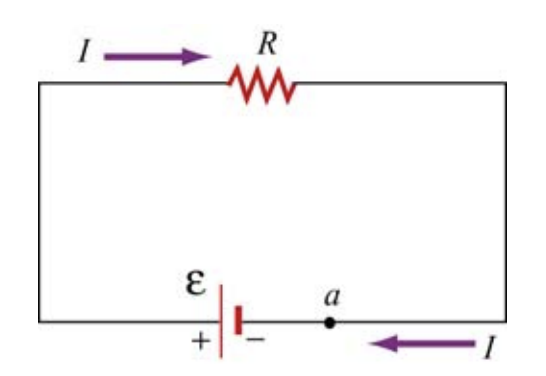
\includegraphics[scale=0.6]{simple}
	\caption{Simple circuit.}
	\label{fig:simple}
\end{figure}

Consider simple circuit consisting of a battery of emf $\mathcal{E}$ and a resistor of resistance $R$ (assuming no internal resistance of the battery). To drive the current, the battery undergoes a discharging process which converts chemical energy to emf. The current $I$ can be found by noting that no work is done in moving a charge $q$ around a closed loop due to the conservative nature of the electrostatic force: \[W = -q\oint\bv{E}\cdot\, d\bv{s} = 0\]

Let point $a$ be the starting point. When crossing from the negative to positive terminal on the battery, the potential increases by $\mathcal{E}$. On the other hand, as we cross the resistor, the potential decreases by an amount $IR$, and the potential energy is converted to thermal in the resistor. Assuming the connecting wire carries no resistance, upon completing the loop, the net change in potential difference must be zero. \[\mathcal{E} - IR = 0 \Rightarrow I = \frac{\mathcal{E}}{R}\] However, the real battery always has an internal resistance (call it $r$), so taking that into account gives us \[\Delta V = \mathcal{E} - Ir\] and because the loop rule still holds, we then have \[\mathcal{E} - Ir - IR = 0\Rightarrow I = \frac{\mathcal{E}}{R + r}\] For a source with emf $\mathcal{E}$, the power or the rate at which energy is delivered is \[P = IR = I(IR + Ir) = I^2R + I^2r\]

\section{Resistors in Series and Parallel.}
\subsection{Series}
Consider a system with a battery with potential difference $\Delta V$ and $n$ resistors connected in series with resistance $R_1, R_2,...,R_n$. 
\begin{figure}[h!]
	\centering
	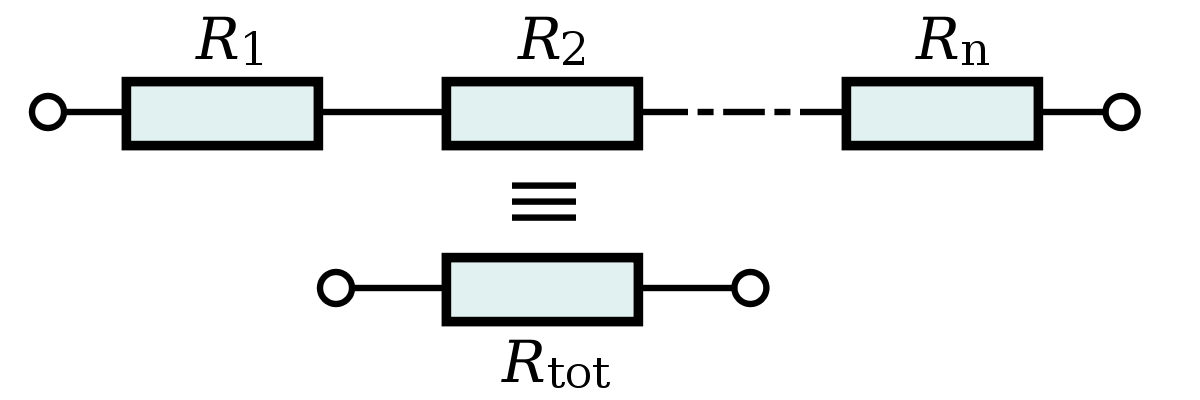
\includegraphics[scale=0.2]{series}
	\caption{$n$ resistors connected in series.}
	\label{fig:series}
\end{figure}

The equivalent resistance of all resistors is thus:
\begin{equation}\label{eqn:series}
	\boxed{R_{eq} = \sum_{i = 1}^{n} R_i}
\end{equation}

\subsection{Parallel}
Consider a system with a battery with potential difference $\Delta V$ and $n$ resistors connected in parallel with resistance $R_1, R_2,...,R_n$.
\begin{figure}[h!]
	\centering
	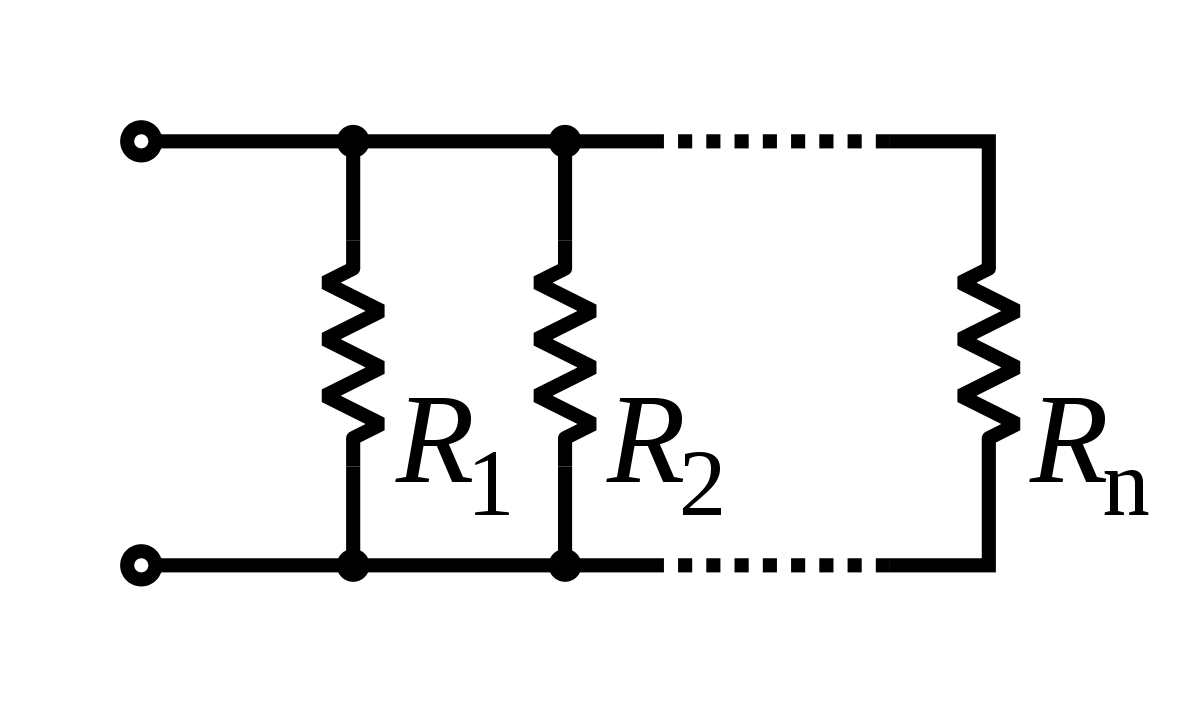
\includegraphics[scale=0.1]{parallel}
	\caption{$n$ resistors connected in parallel.}
	\label{fig:parallel}
\end{figure}

The equivalent resistance of all resistors is thus:
\begin{equation}\label{eqn:parallel}
	\boxed{\frac{1}{R_{eq}} = \sum_{i = 1}^{n} \frac{1}{R_i}}
\end{equation}

\section{Kirchhoff's Circuit Rules.}
In analyzing circuits, we have two fundamental rules called Kirchhoff's rules :
\begin{itemize}
	\item Junction Rule: 
	
	At any point where there is a junction between various current carrying branches, by current conservation the sum of the currents into the node must be equal to the sum of the currents out of the node (otherwise charge would build up at the junction instead of free-flowing): \[\sum I_{in} = \sum I_{out}\]
	\item Loop Rule:
	
	The sum of the voltage drops $\Delta V_i$, across any circuit elements that form a closed circuit is zero: \[\sum_{\text{closed loop}}\Delta V_i = 0\]
\end{itemize}

\textbf{Note}. When deciding the sign of $\Delta V_i$ for a given circuit element, just remember that, with a given direction, $\Delta V_i$ would be negative to go from higher to lower potential, positive vice versa.

\section{RC Circuits.}
\subsection{Charging}
Consider the following circuit. At time $t = 0$, the switch $S$ is closed. The capacitor initially is uncharged, i.e. $q(t = 0) = 0$. 
\begin{figure}[h!]
	\centering
	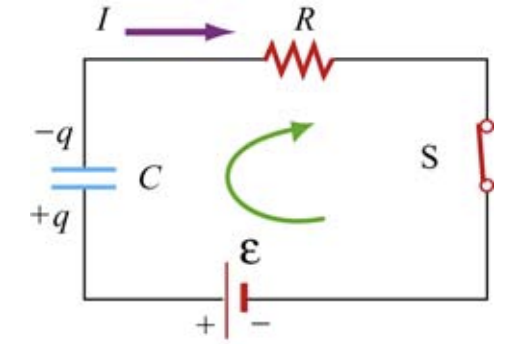
\includegraphics[scale=0.5]{rc}
	\caption{Simple $RC$ circuit with a switch.}
	\label{fig:rc}
\end{figure}

In particular for $t < 0$, there is no voltage across the capacitor so the capacitor acts like a short circuit (a straight wire). At $t = 0$, the switch is closed and current begins to flow according to \[I_0 = \frac{\mathcal{E}}{R}\] At this moment, the potential difference from the battery terminals is the same as that across the resistor. This initiated the charging of the capacitor. As the capacitor begins to charge, the voltage across the capacitor increases with time: \[V_C(t) = \frac{q(t)}{C}\] Using Kirchhoff's loop rule for capacitors and traversing the loop clockwise, we obtain
\begin{align*}
	0  & = \mathcal{E} - I(t)R - V_C(t)\\
		& = \mathcal{E} - \frac{dq}{dt}R - \frac{q}{C}
\end{align*}

Since $I$ must be the same in all parts of the series circuit, the current across the resistance $R$ is equal to the rate of increase of charge on the capacitor plates. The current flow in the circuit will continue to decrease because the charge already present on the capacitor make sit harder to put more charge on it. Once the charge on the capacitor plates reaches its maximum value $Q$, the current in the circuit drops to $0$: \[I(t)R = \mathcal{E} - V_C(t)\] Thus, the charging capacitor follows a first-order differential equation that relates the rate of change of charge to the charge on the capacitor: \[\frac{dq}{dt} = \frac{1}{R}\left(\mathcal{E} - \frac{q}{C}\right)\] Differential equations of the form can generally be solved with separation of variables (putting terms involving $dq$ and $q$ on one side and terms involving $dt$ on the other side): \[\frac{dq}{\left(\mathcal{E} - \frac{q}{C}\right)} = \frac{1}{R}dt \,\Rightarrow \frac{dq}{q - C\mathcal{E}} = -\frac{1}{RC}dt\] Perform integration on each side respectively: \[\int_0^q\frac{dq'}{q'-C\mathcal{E}} = -\frac{1}{RC}\int_0^tdt'\] which gives us \[ln\left(\frac{q - C\mathcal{E}}{-C\mathcal{E}}\right) = -\frac{t}{RC}\] Now, simplify the equation yields:
\begin{equation}\label{eqn:charging}
	\boxed{q(t) = C\mathcal{E}\left(1 - e^{-t/RC}\right) = Q(1 - e^{(-t/RC)}}
\end{equation}

where $Q = RC$ is the maximum amount of charge stored on the plates. The time dependence of $q(t)$ is shown below:\newpage
\begin{figure}[h!]
	\centering
	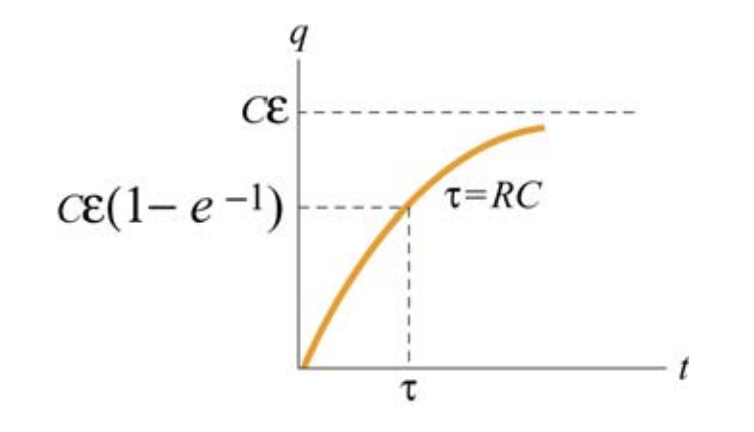
\includegraphics[scale=0.4]{charge-graph}
	\caption{Charge as a function of time during charging process.}
	\label{fig:charging}
\end{figure}

Now we can derive related quantities as well, such as voltage $V_C(t)$ across the capacitor: \[V_C(t) = \frac{q(t)}{C} = \mathcal{E}(1 - e^{-t/RC})\] or the current in the system: \[I(t) = \frac{dq}{dt} = \left(\frac{\mathcal{E}}{R}\right)e^{-t/RC} = I_0e^{-t/RC}\] We give $RC$ a fancy name: \textbf{time constant}. The SI units of $\tau$ are seconds. It is a measure of the decay time for the exponential function. This decay rate satisfies the following property: \[I(t+\tau) = I(t)e^{-1}\]

\subsection{Discharging}
Now, suppose that the capacitor has been charged to some value $Q$, the switch is open and the potential difference across the capacitor is given by $V_C = Q/C$, and no current is flowing. Now, close the switch at $t = 0$, the capacitor will discharge to decrease its energy.
\begin{figure}[h!]
	\centering
	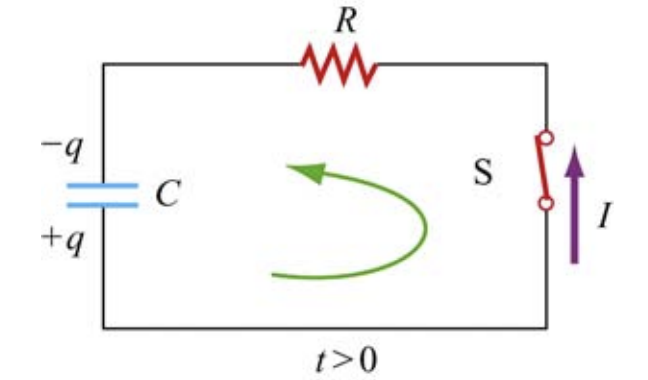
\includegraphics[scale=0.5]{discharge}
	\caption{Capacitor discharges.}
	\label{fig:discharge}
\end{figure}

I will leave the derivation and graphing as an exercise for the reader.

\section{Exercises.}
\subsection{Warm-up}
%7.9.3
\textbf{Problem 1}. In the circuit below, suppose the switch has been open for a very long time. At time $t = 0$, it is suddenly closed.

\begin{itemize}
	\item What is the time constant before the switch is closed?
	\item What is the time constant after the switch is closed?
	\item Find the current through the switch as a function of time after the switch is closed.
\end{itemize}
\begin{figure}[h!]
	\centering
	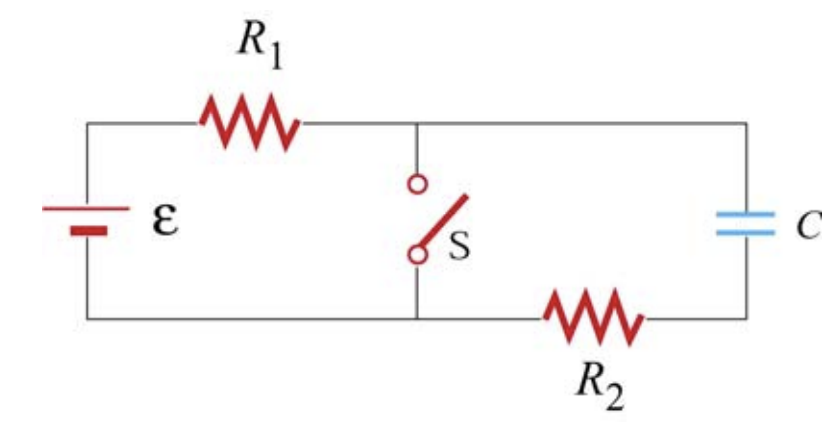
\includegraphics[scale=0.5]{p1}
	\caption{RC circuit network.}
	\label{fig:p1}
\end{figure}

\subsection{Conceptual Questions}
%7.10.2-4
\textbf{Problem 2}. Why do the headlights on cars become dim when the car is starting?

\textbf{Problem 3}.Does the resistor in an RC circuit affect the maximum amount of charge that can be stored in a capacitor? Explain.

\textbf{Problem 4}. Can one construct a circuit such that the potential difference across the terminals of the battery is zero? Explain.
\newpage
\subsection{More Practice}
%7.11.2
\textbf{Problem 5}. Consider the following network. Neglecting the internal resistance of the batteries, calculate the currents through each of the three resistors.
\begin{figure}[h!]
	\centering
	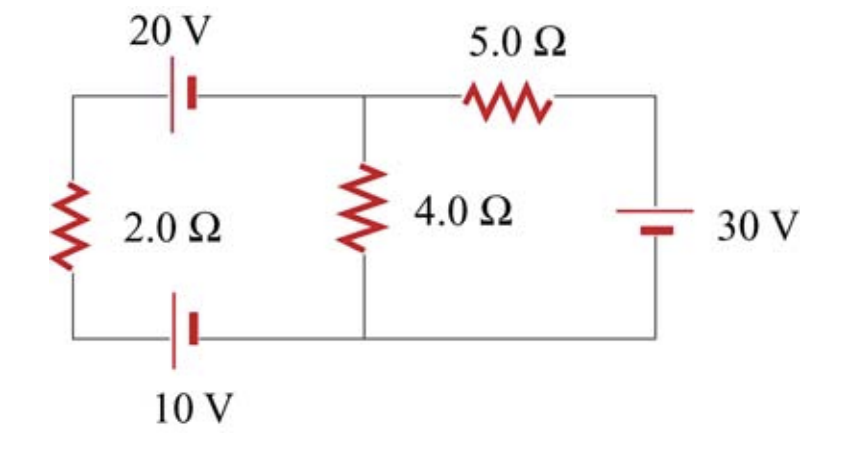
\includegraphics[scale=0.4]{p2}
	\caption{(Another) RC circuit network.}
	\label{fig:p2}
\end{figure}

%7.11.4
\textbf{Problem 6}. Consider an infinite network of resistors of resistances $R_0$ and $R_1$ shown below. Find $R_{eq}$.
\begin{figure}[h!]
	\centering
	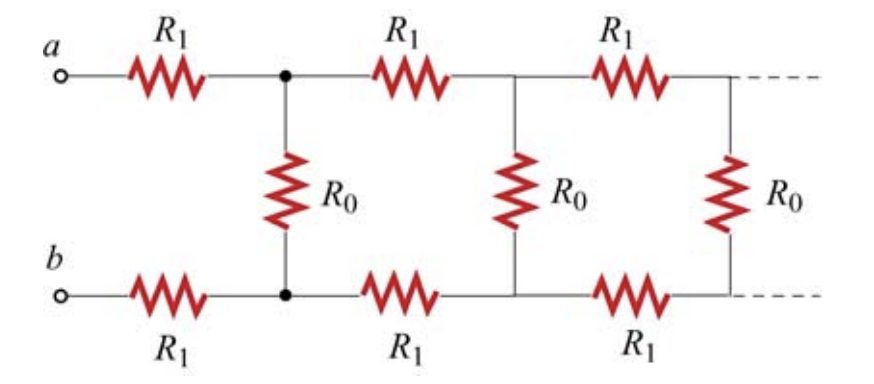
\includegraphics[scale=0.45]{p3}
	\caption{Resistor chain.}
	\label{fig:p3}
\end{figure}

%Irodov 
\textbf{Problem 7}. A cylindrical capacitor connected to a DC voltage source $V$ touches the surface of water with its end. The separation $d$ between the capacitor electrodes is substantially less than their mean radius. Find a height $h$ to which the water level in the gap
will rise. The capillary effects are to be neglected.
\begin{figure}[h!]
	\centering
	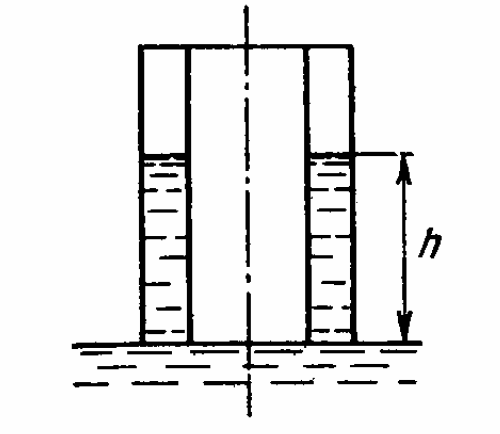
\includegraphics[scale=0.45]{p4}
	\caption{Capacitor touching water.}
	\label{fig:p4}
\end{figure}

\end{document}
